\chapter{Variable gear-ratio actuation technology}
\label{sec:MultipleSpeedActuationTechnology}

\section{Requirements}
\label{sec:Requirements}

\begin{figure}[H]
	\centering
		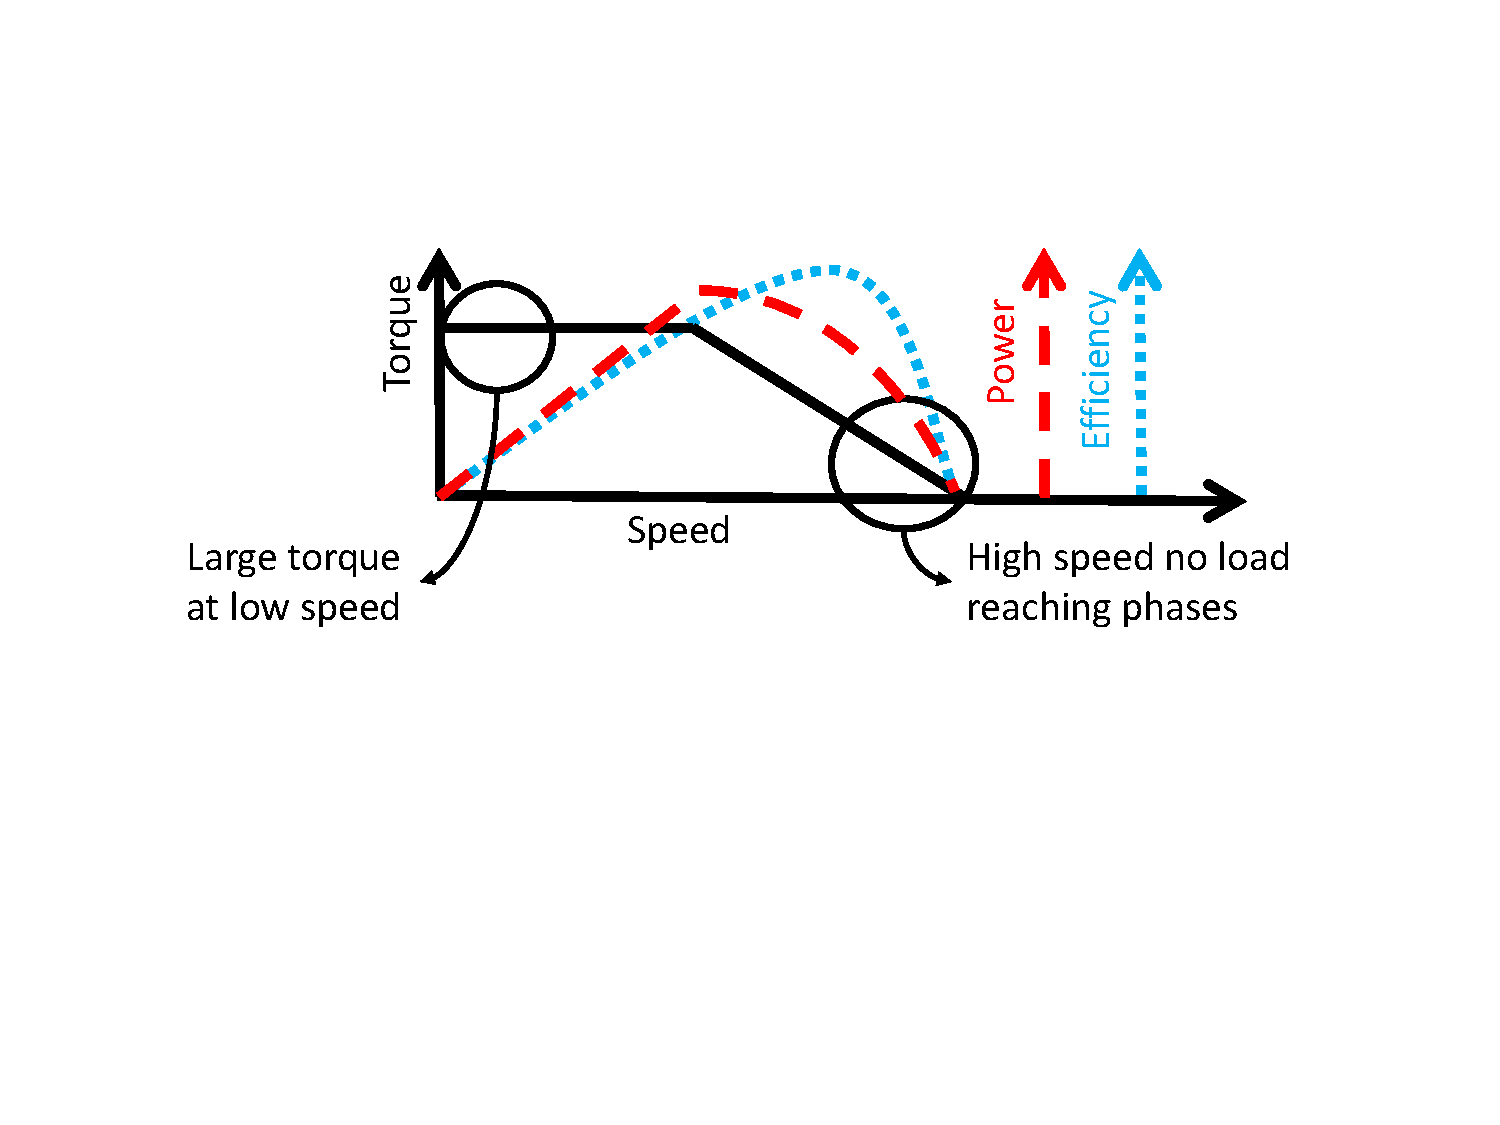
\includegraphics[width=0.45\textwidth]{speedissue.pdf}
	\caption{Limitations of EM motors for extremum torque-speed operations}
	\label{fig:speedissue}
\end{figure}

\section{Actuator Research}
\label{sec:actres}

Traditional robots generally use actuators that behave as displacement-sources because of their high intrinsic impedance. These include geared EM motors and hydraulics cylinders. Using a force sensor, it is possible to control the output force using those actuators, but the bandwidth is rather limited. To guarantee the stability of the force-feedback scheme only half the intrinsic inertia can be canceled \cite{hogan_impedance_2004}. Since 70's, roboticists have been attempting to build actuators that can behave naturally as a force-source such as series-elastic actuators, pneumatic cylinder and air-muscles \cite{hanafusa_stable_1977}\cite{pratt_series_1995}. However, because of the physical limitation of compliant transmission materials, the achievable bandwidth is limited and precise position control is hardly achievable. Direct drive EM actuators are the best force-source actuators with high fidelity, high bandwidth. However, the very low force density and low efficiency at low speeds make them impractical for mobile robot applications \cite{hollerbach_comparative_1992}. Moreover, on the other hand, actuators with non-back-drivable mechanisms have the advantage for pure position control tasks and they can bear very large load without any power consumption.

Since both small and large intrinsic impedances are advantageous in different scenario, several group have developed variable intrinsic impedance actuators, such as based on variable stiffness spring \cite{tonietti_design_2005}, antagonist non-linear devices \cite{koganezawa_antagonistic_2006}, a series-compliance that can be locked with a brake \cite{leach_linear_2012} and dual-motors in serial configuration \cite{kim_serial-type_2010}. Furthermore, so-called macro-micro actuators, can improve the bandwidth of force-source type of actuators by exploiting the high-bandwidth of a small actuator in parallel, allowing for wider-range impedance control and improved position control \cite{morrell_parallel-coupled_1998}.

While the actuator work in robotics have been focused on impedance and bandwidth issues, in the powertrain field the torque-speed matching issue is predominant, since power density and efficiency are critical for mobile systems.


\section{Dual-Speed Dual-Motor architecture}
\label{sec:DSDM}


\begin{figure}[H]
	\centering
		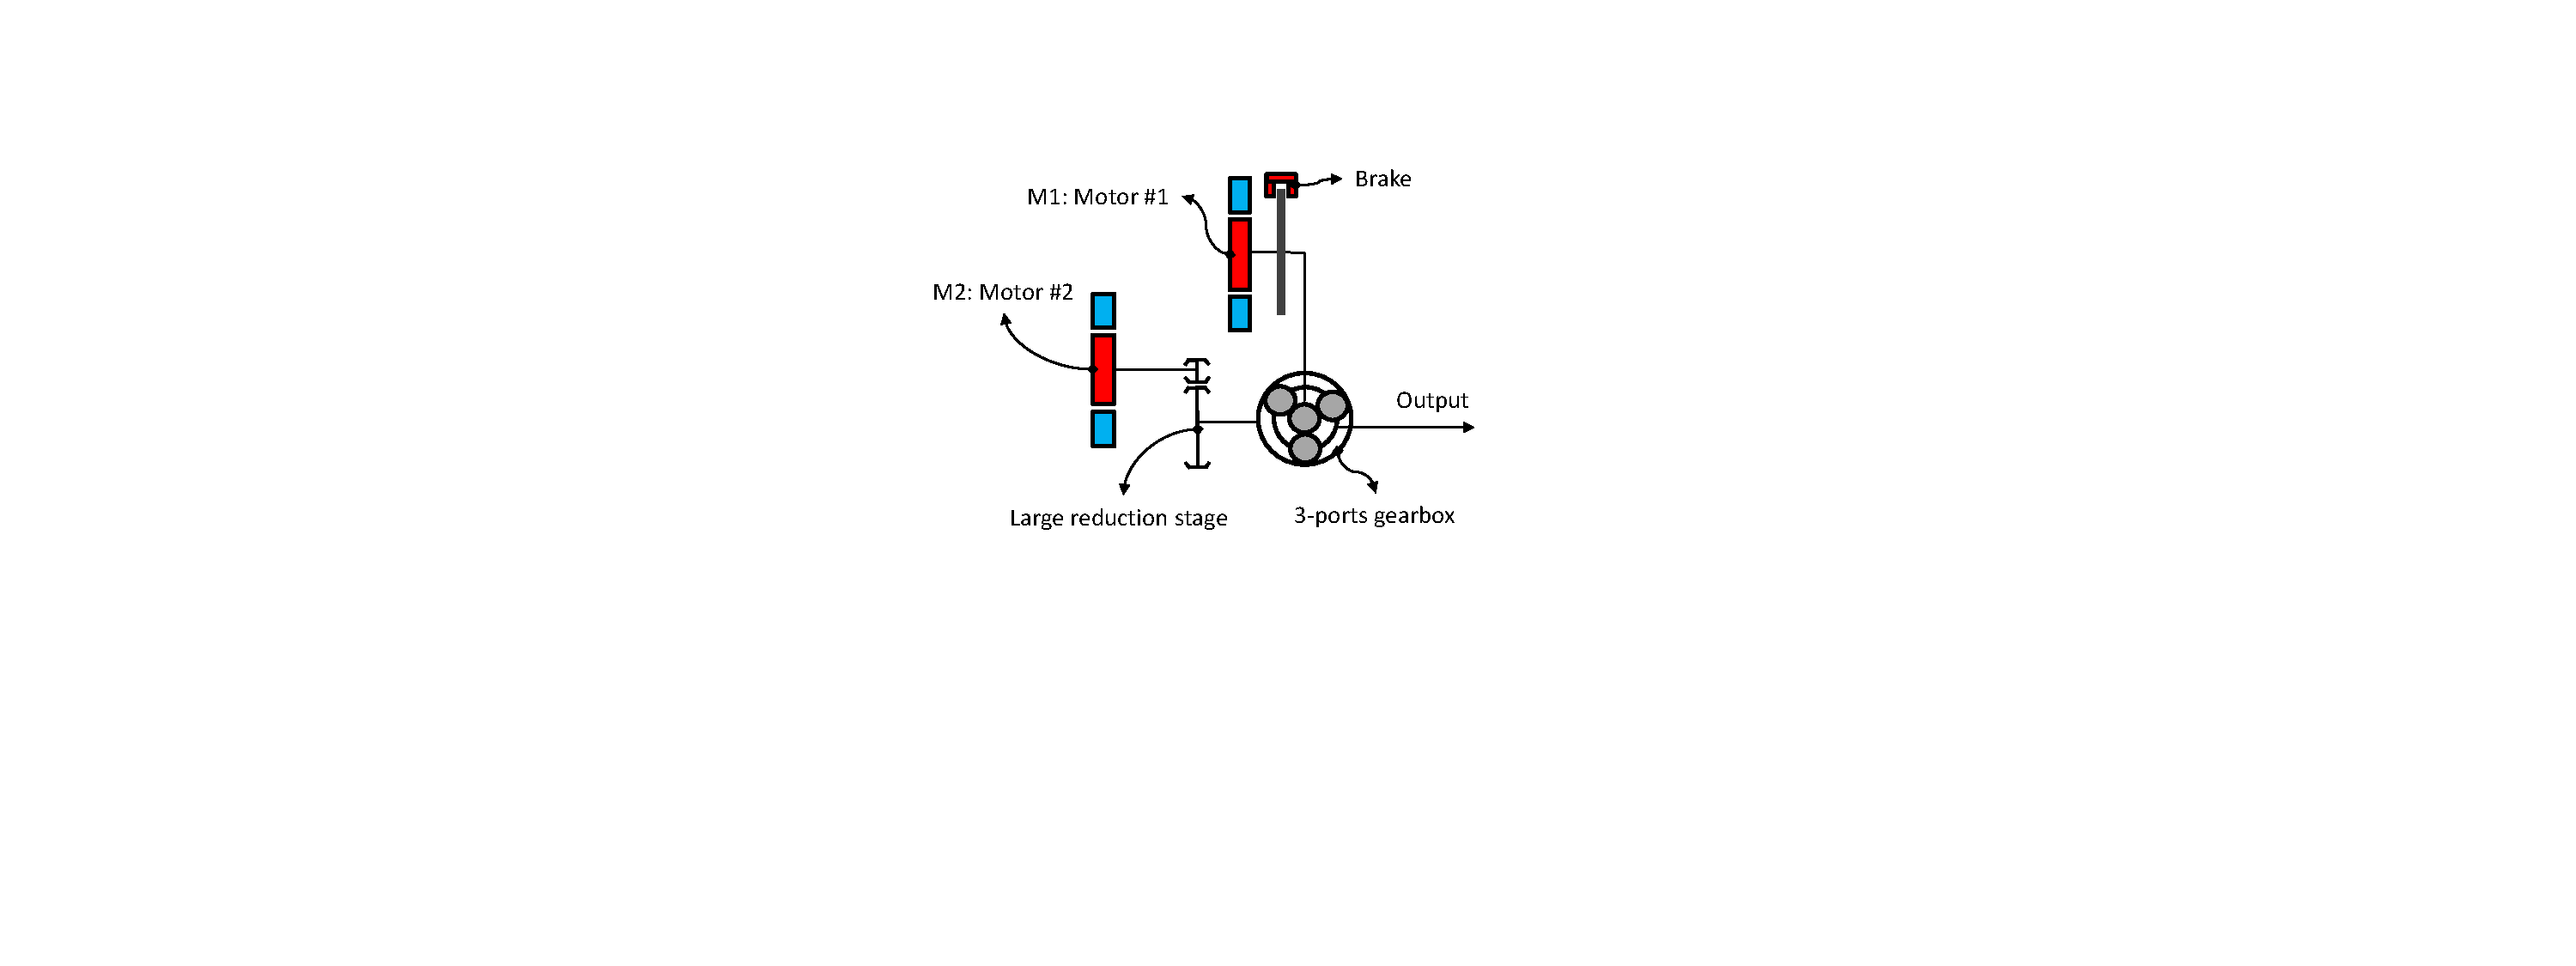
\includegraphics[width=0.40\textwidth]{dualmotorconcept2.pdf}
	\caption{DSDM actuator concept}
	\label{fig:dualmotorconcept}
\end{figure}


\begin{figure}[H]
	\centering
		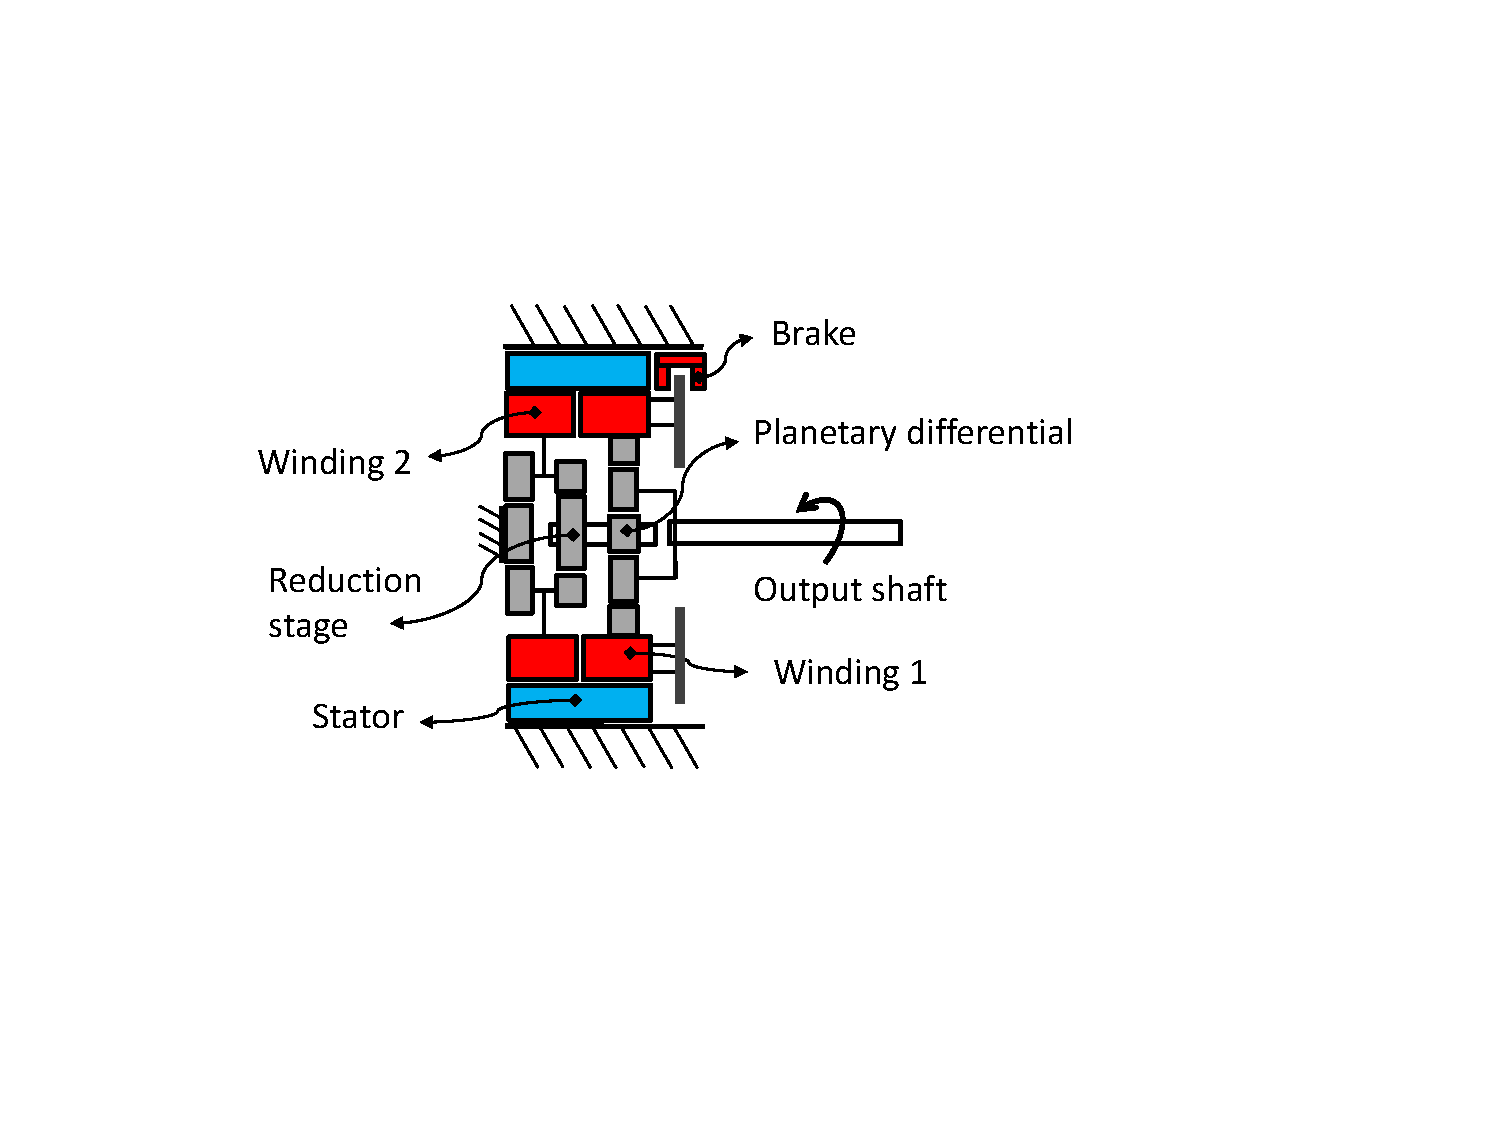
\includegraphics[width=0.40\textwidth]{embedded3.pdf}
	\caption{Possible architecture of an integrated DSDM concept}
	\label{fig:embedded}
\end{figure}


\begin{figure}[H]
	\centering
		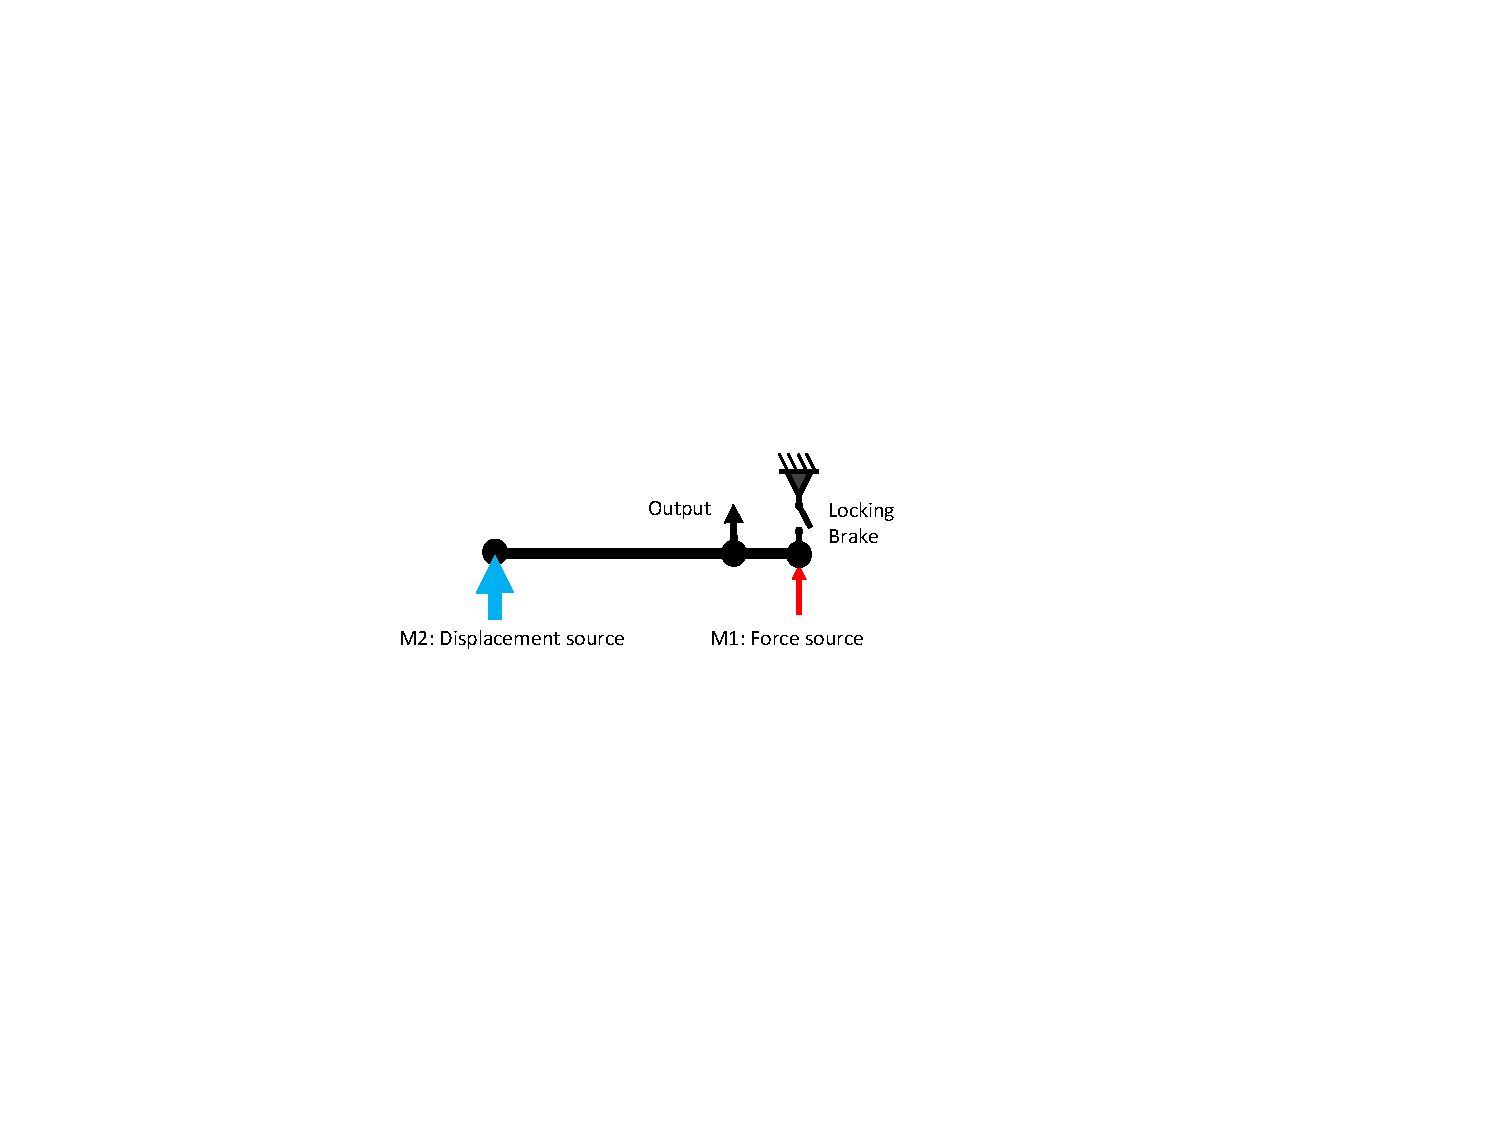
\includegraphics[width=0.40\textwidth]{lever.pdf}
	\caption{Dual input system}
	\label{fig:lever}
\end{figure}
%
\begin{figure}[H]
        \centering
				\subfloat[High force mode (brake closed)]{
        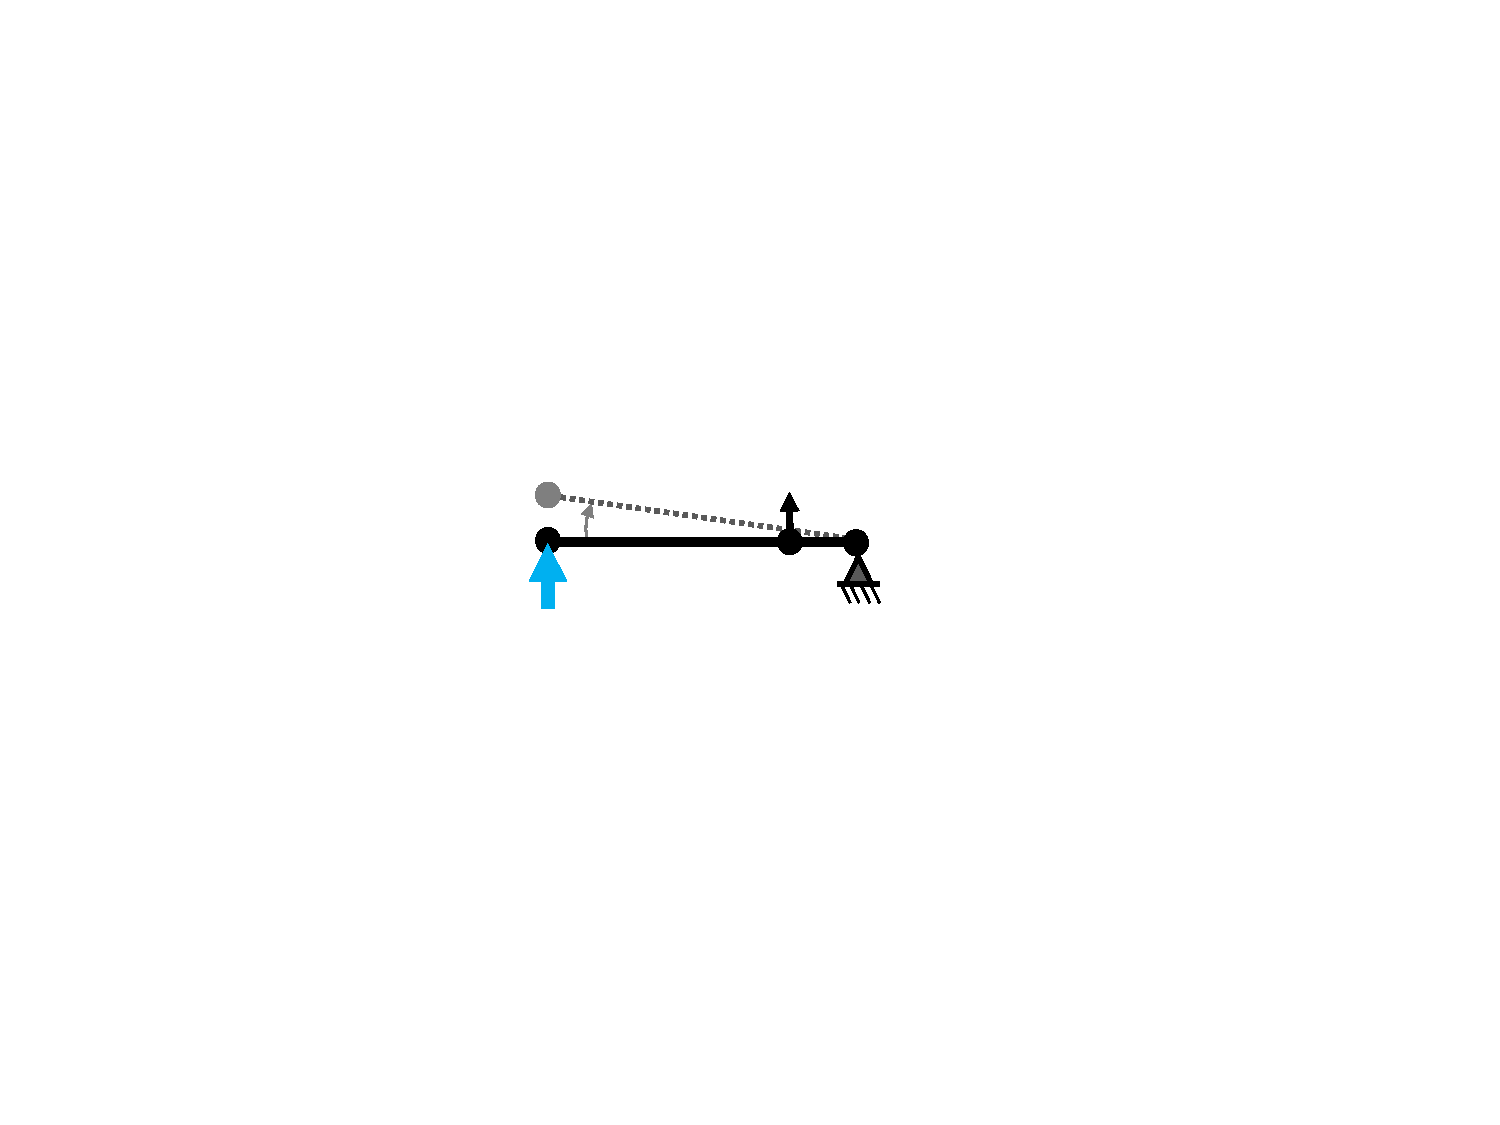
\includegraphics[width=0.22\textwidth]{leverHF.pdf}
				\label{fig:HF}}
        \subfloat[High speed mode (brake open)]{
				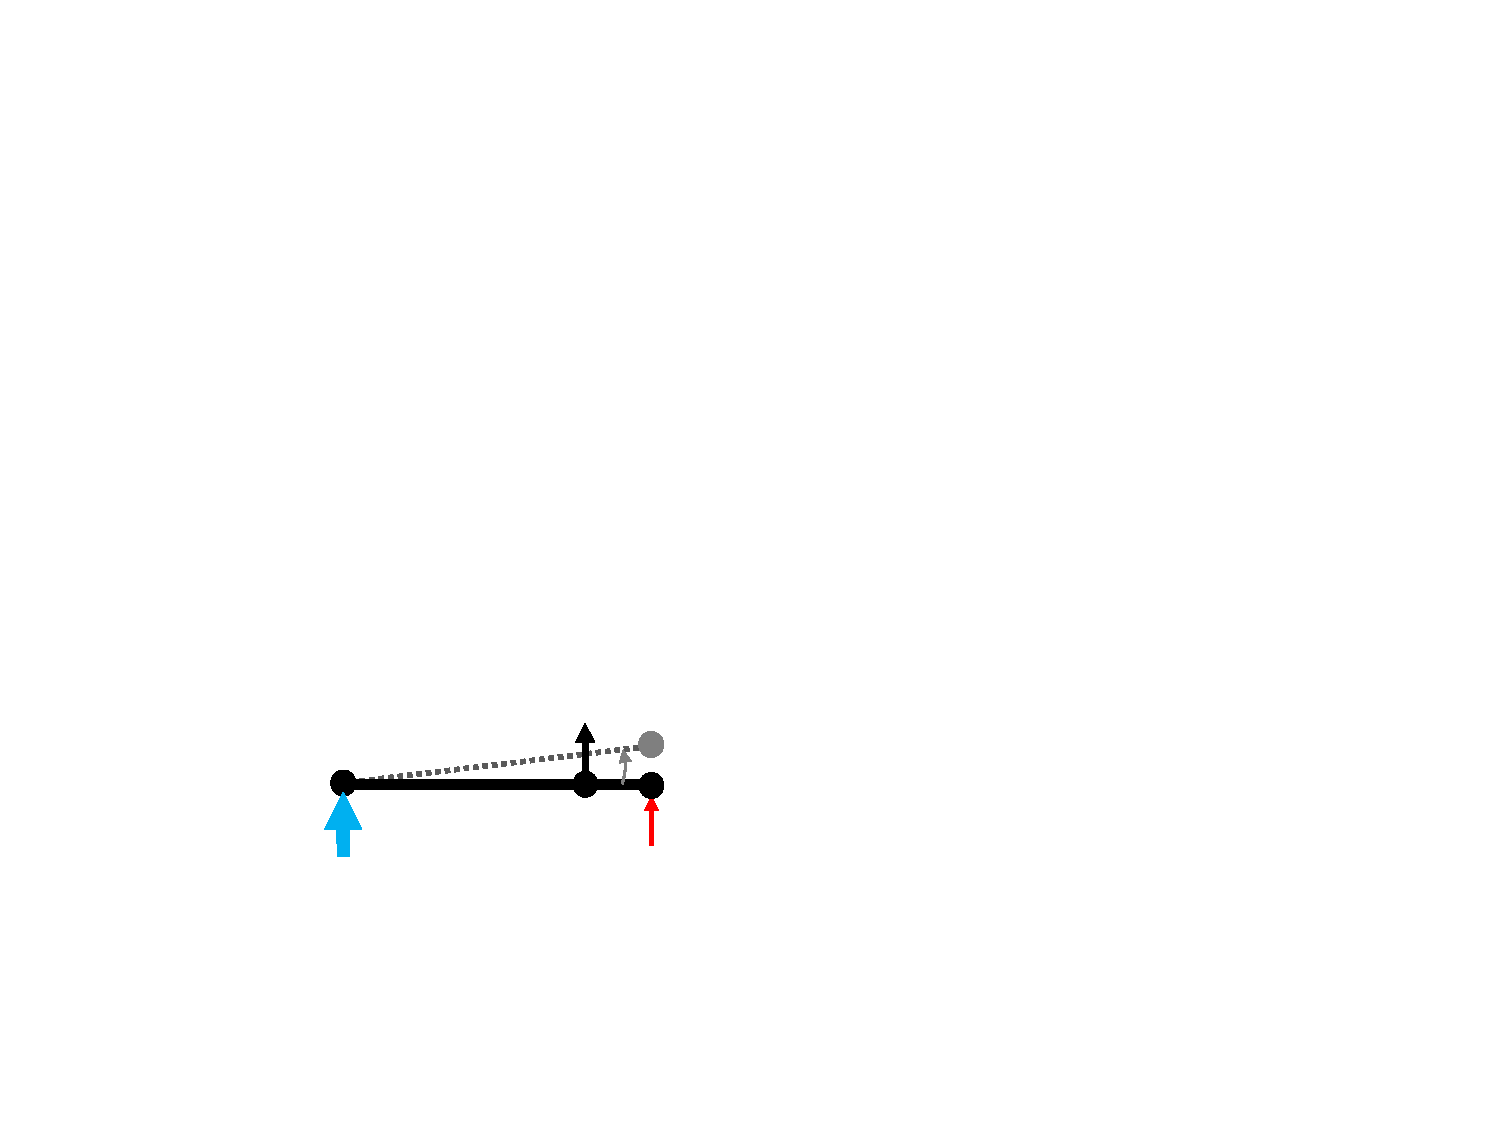
\includegraphics[width=0.22\textwidth]{leverHS.pdf}
				\label{fig:HS}}
        \caption{Two modes of operation}\label{fig:opmode}
\end{figure}

\begin{figure}[H]
	\centering
		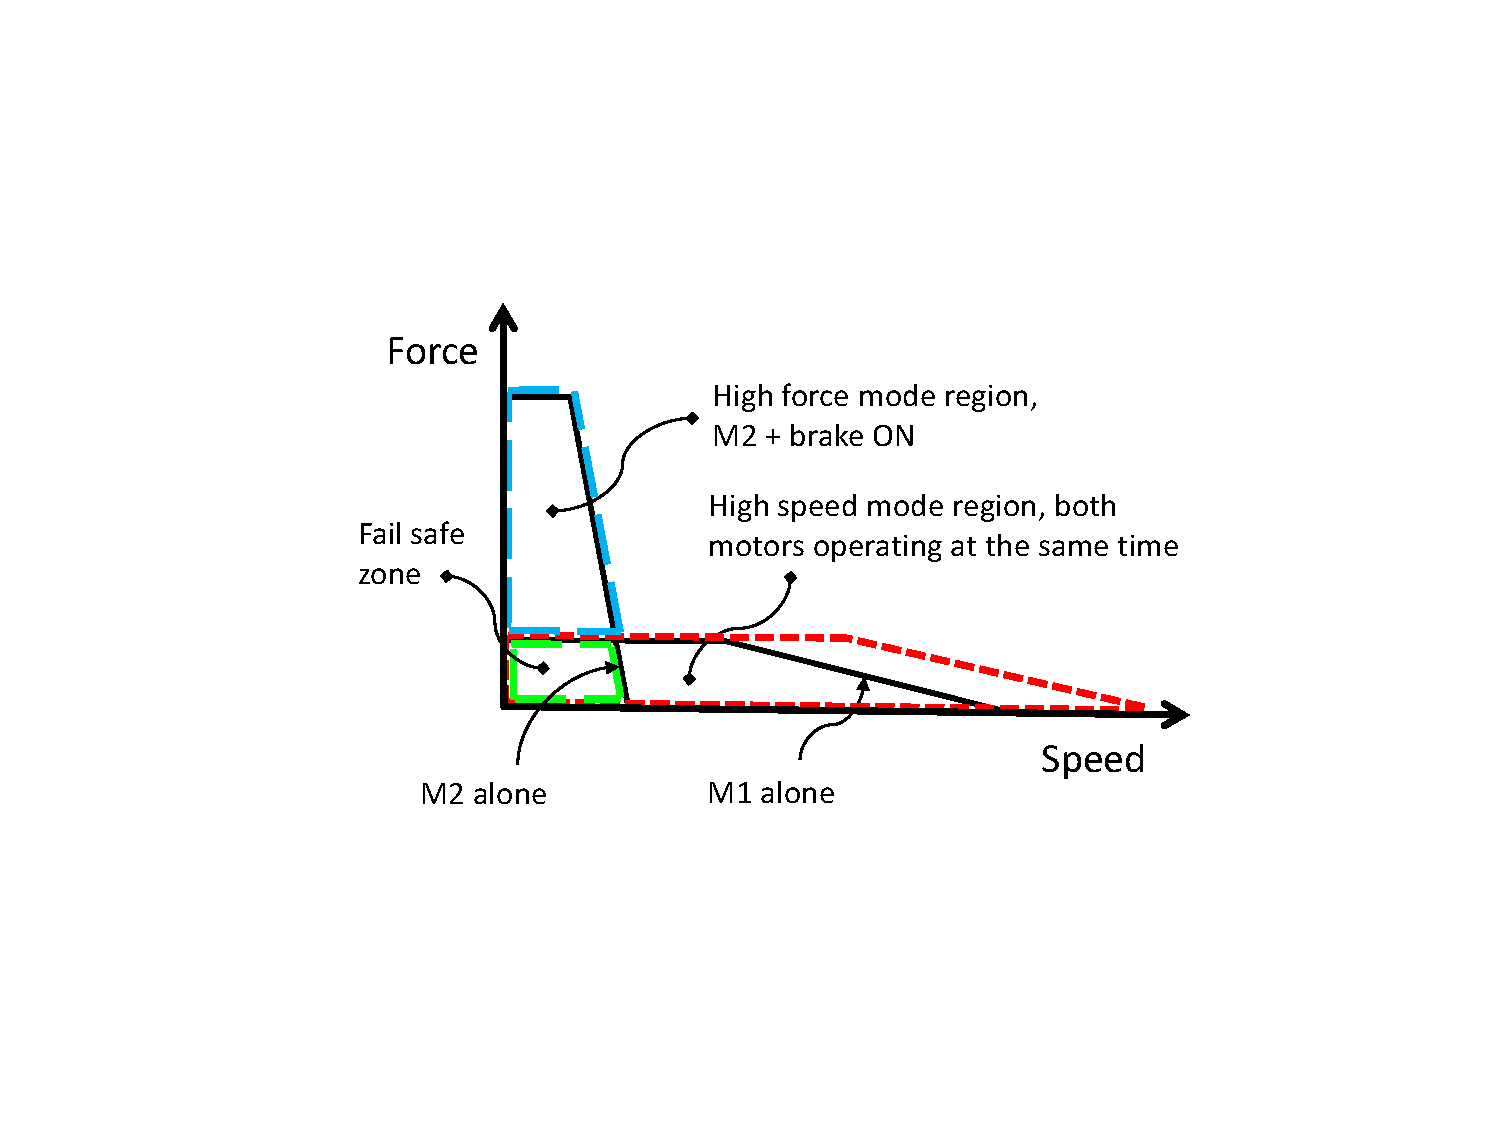
\includegraphics[width=0.45\textwidth]{torquespeed.pdf}
	\caption{DSDM actuator operation region, with a difference between M1 and M2 gearing ratio of only 4 for illustration purposes }
	\label{fig:torquespeed}
\end{figure}


\begin{figure}[H]
        \centering
				\subfloat[One motor solution]{
				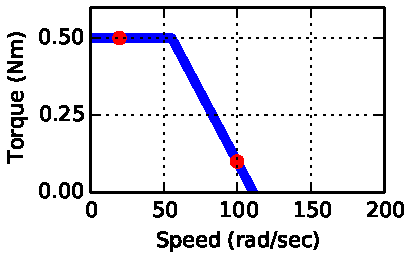
\includegraphics[width=0.22\textwidth]{sol1.pdf}
				\label{fig:s1}}
        \subfloat[DSDM solution]{
				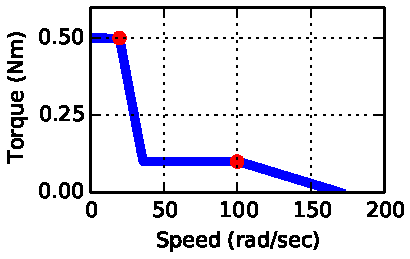
\includegraphics[width=0.22\textwidth]{sol2.pdf}
				\label{fig:s2}}
        \caption{Case study of two actuator solution for two 10 W operating points }\label{fig:solutions}
\end{figure}

\begin{figure}[H]
	\centering
		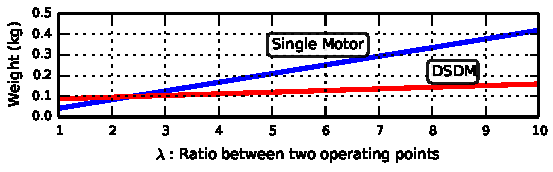
\includegraphics[width=0.45\textwidth]{w_vs_ratio.pdf}
	\caption{Weight of a single motor compared to the DSDM concept for two 10 W operating points at different speeds $w_1=100$ rad/sec, $w_2 = w_1 / \lambda$}
	\label{fig:1vs2}
\end{figure}


\section{Fast and Seamless gearshifts}
\label{sec:FastAndSeamlessGearshifts}

\begin{figure}[H]
	\centering
		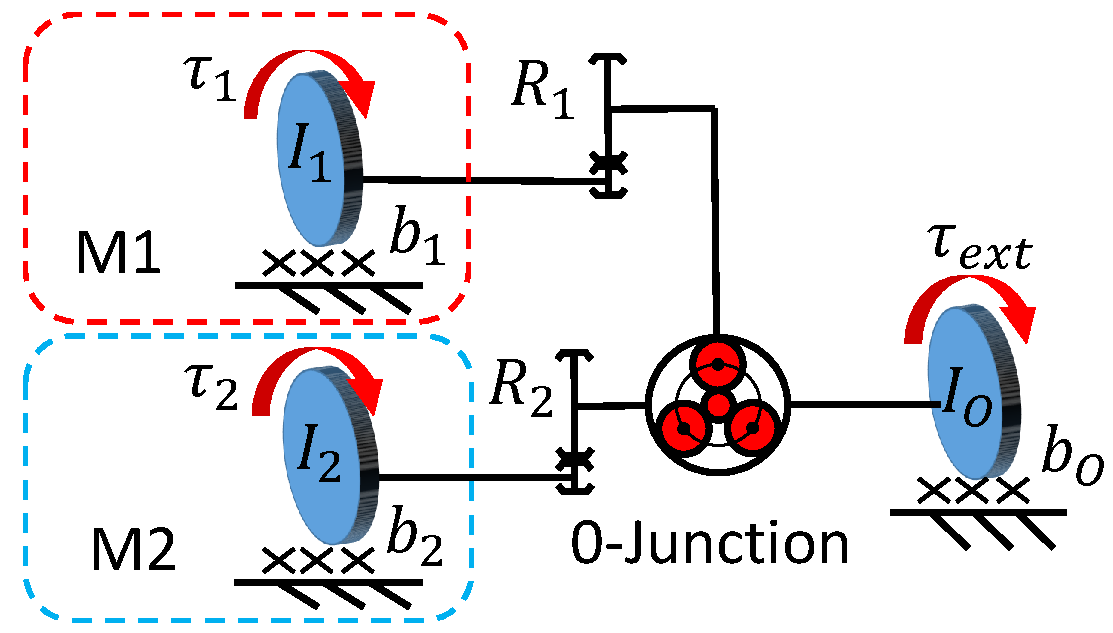
\includegraphics[width=0.45\textwidth]{dynamics.pdf}
	\caption{Lumped-parameter dynamic model of a DSDM}
	\label{fig:dynamics}
\end{figure}

\begin{figure}[H]
	\centering
		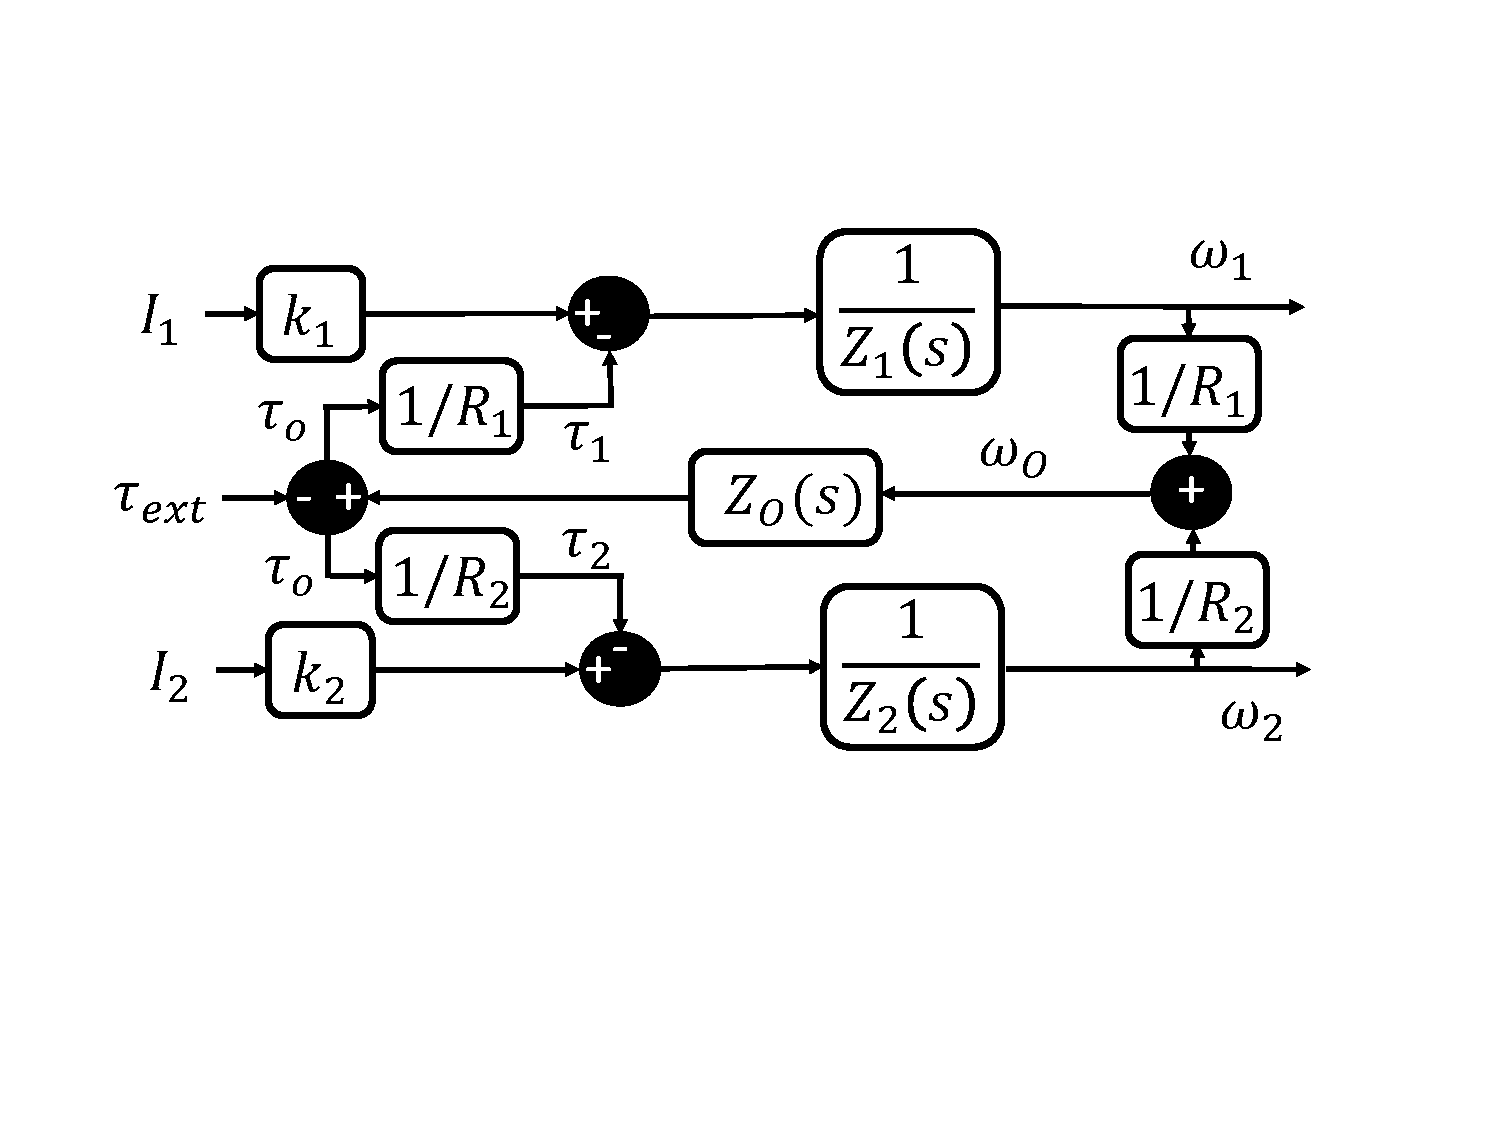
\includegraphics[width=0.40\textwidth]{dynamics_block.pdf}
	\caption{Dynamics of a DSDM}
	\label{fig:dynamics_block}
\end{figure}

\subsection{Nullspace of the system}

\subsection{Control Algorithm}


\begin{figure}[H]
	\centering
		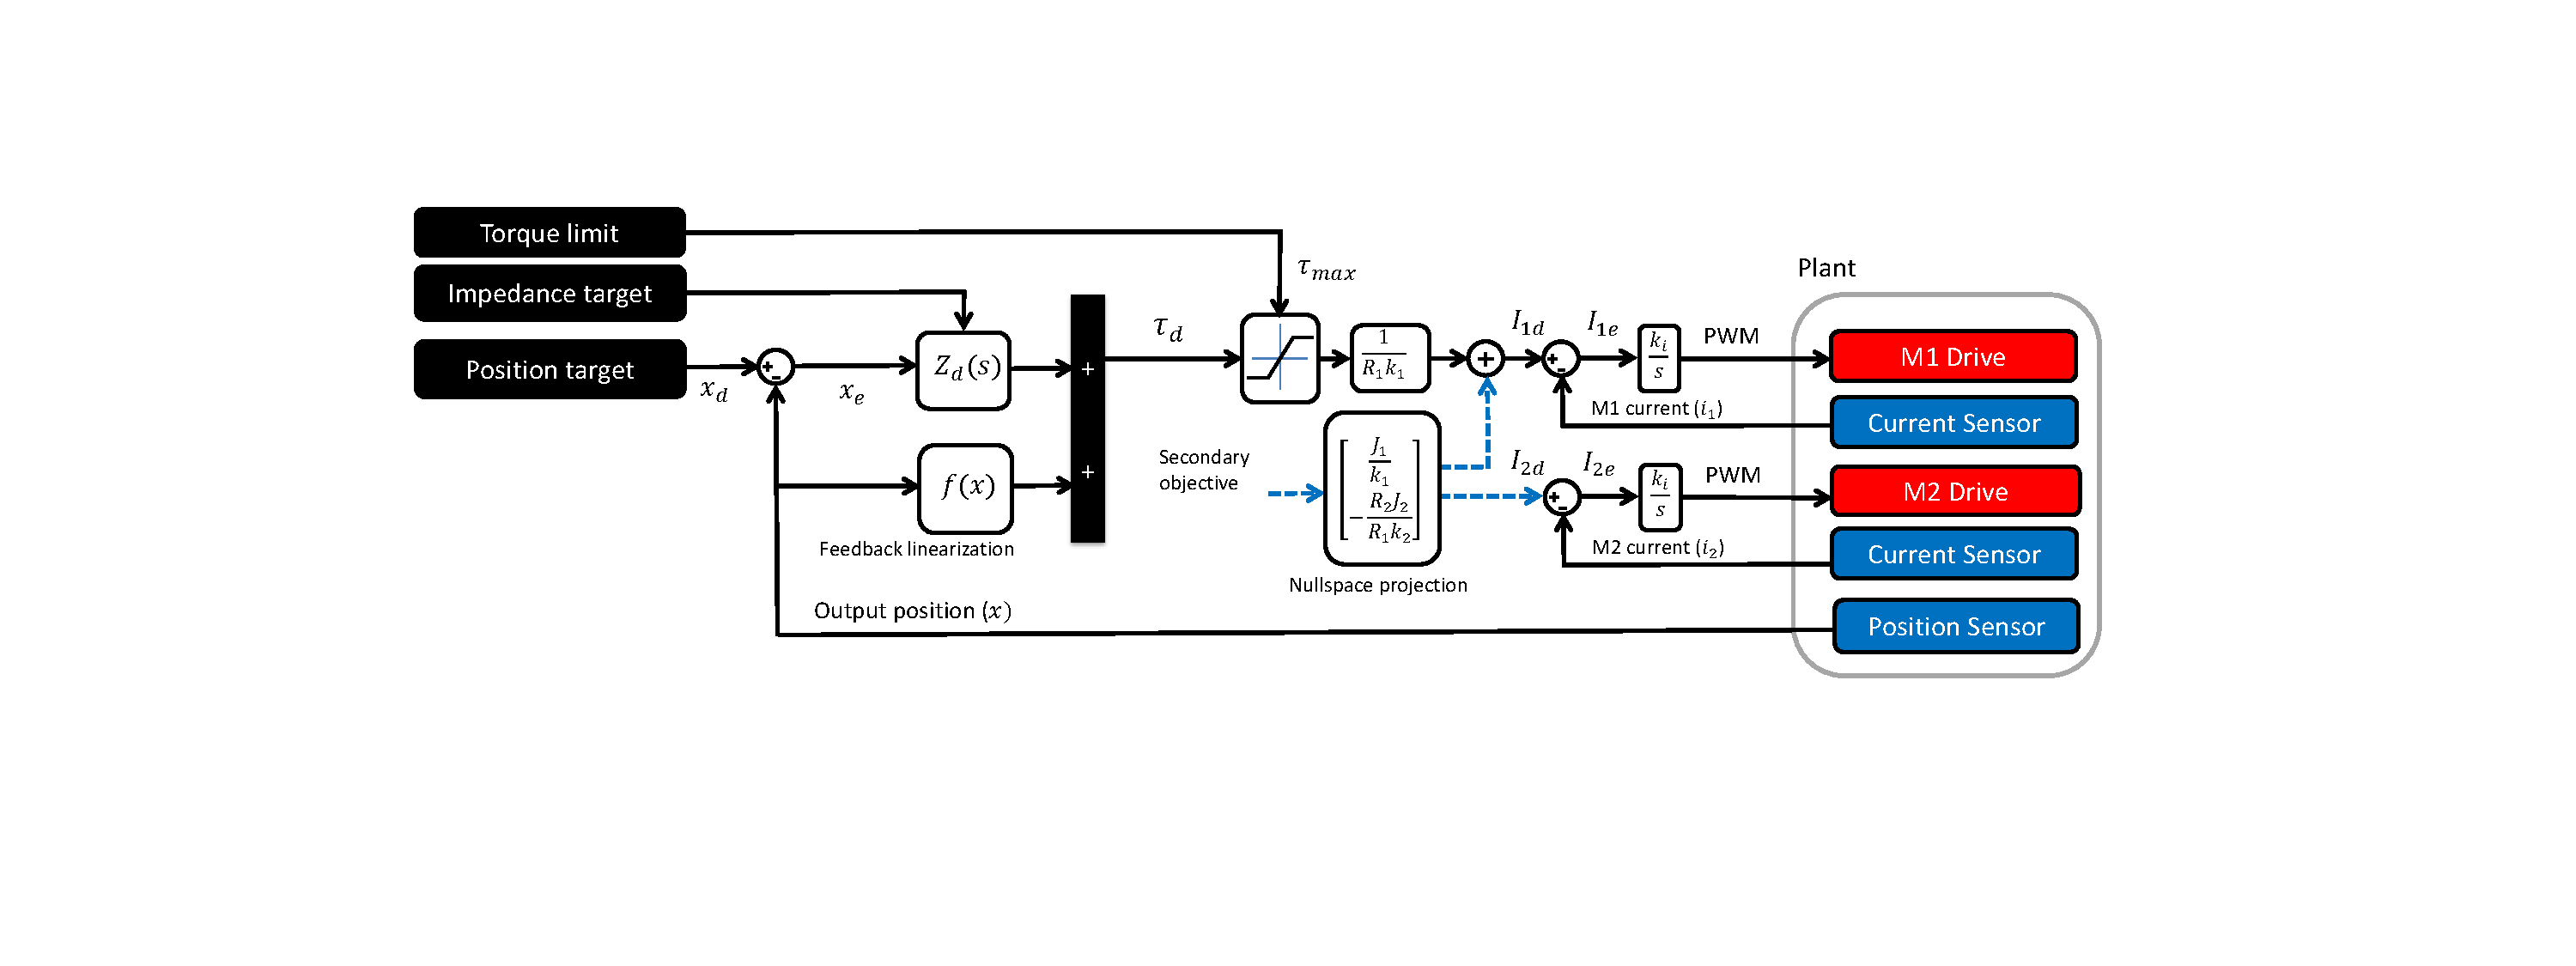
\includegraphics[width=1.00\textwidth]{HS_loop.pdf}
	\caption{High-speed mode control loop}
	\label{fig:HS_loop}
\end{figure}

\begin{figure}[H]
	\centering
		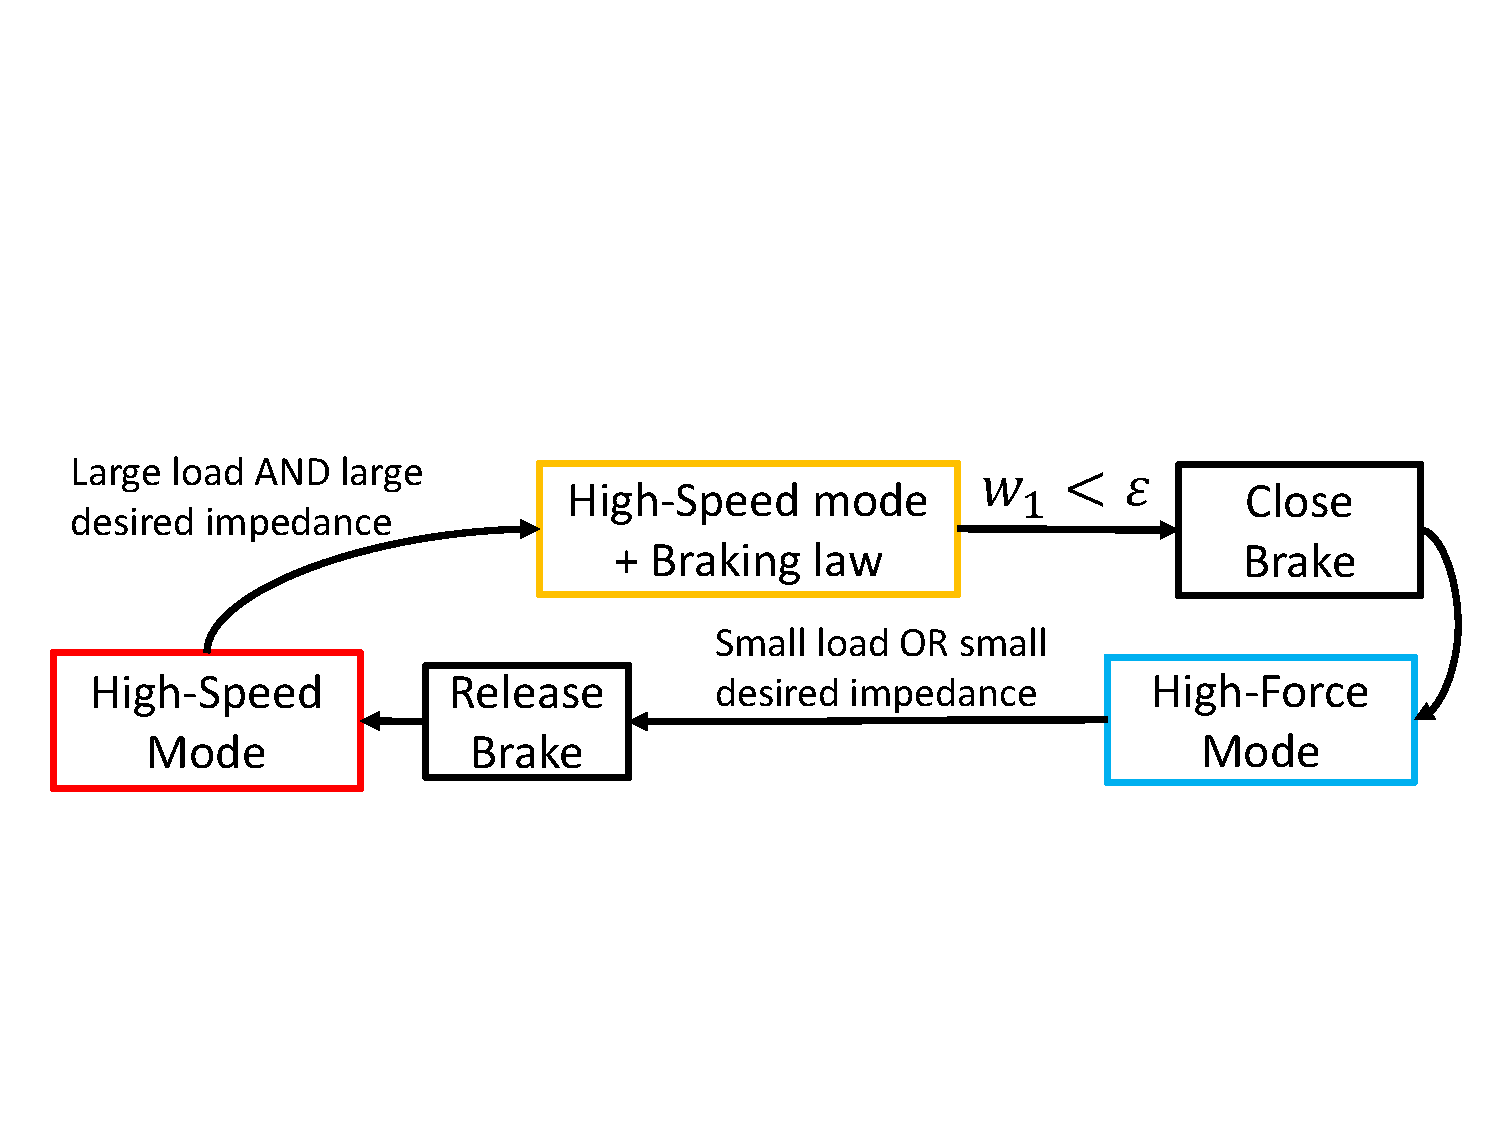
\includegraphics[width=0.45\textwidth]{automatic_flow.pdf}
	\caption{State machine for automatic mode selection}
	\label{fig:automaticflow}
\end{figure}


\subsection{Using impact forces for faster transitions}


